\documentclass[a4paper,14pt]{extarticle}

\usepackage{geometry}
\usepackage{amsmath,bm}
\usepackage{amssymb}
\usepackage{amsthm}
\usepackage{esint}
\usepackage{float}
\usepackage{graphicx}
\usepackage[dvipsnames]{xcolor}
\usepackage[utf8]{inputenc}
\usepackage[T2A]{fontenc}
%\usepackage[lutf8x]{luainputenc}

%\usepackage{fontspec}
%\setmainfont{CMU Serif}
%\setsansfont{CMU Sans Serif}
%\setmonofont{CMU Typewriter Text}

\usepackage[greek.polutoniko,english,russian]{babel}
% локализация и переносы
\usepackage{latexsym}
\usepackage{hhline}
\usepackage{multirow}
\usepackage{vmargin,indentfirst} 
\setmarginsrb{20mm}{15mm}{15mm}{15mm}{0mm}{0mm}{0mm}{10mm}
\usepackage[multiple]{footmisc}
\usepackage{hyperref}
\usepackage{multirow}
\usepackage{pdflscape}
%\numberwithin{equation}{section}
\usepackage[labelsep=period]{caption}


% команда для переноса строки внутри ячейки таблицы
\newcommand{\specialcell}[2][l]{%
  \begin{tabular}[#1]{@{}l@{}}#2\end{tabular}}

  \usepackage{physics}

\usepackage{tikz}
\usetikzlibrary{calc}
\usetikzlibrary{arrows.meta}

%\usepackage[margin=0.3in,bmargin=0.5in]{geometry}

%\usepackage{CJKutf8}%Chinese characters


\pagestyle{plain}

\theoremstyle{plain}
\newtheorem{theorem}{Theorem}[section]
\newtheorem{lemma}[theorem]{Lemma}
\newtheorem*{proposition}{Proposition}
\newtheorem{corollary}[theorem]{Corollary}
\newtheorem{problem}[theorem]{Problem}
\newtheorem{exercise}{Exercise}[section]

\theoremstyle{remark}
\newtheorem*{example}{Example}
\newtheorem*{examples}{Examples}
\newtheorem*{remark}{Remark}
\newtheorem*{hint}{Hint}

\theoremstyle{definition}
\newtheorem*{definition}{Definition}

\renewcommand{\emptyset}{\varnothing}
\newcommand\ph{\varphi}
\newcommand\eps{\varepsilon}

\newcommand\mbZ{\mathbb Z}
\newcommand\mbC{\mathbb C}
\newcommand\mbR{\mathbb R}
\newcommand\mbN{\mathbb N}
\newcommand\mbQ{\mathbb Q}
\newcommand\mbE{\mathbb E}

\newcommand\mcB{\mathcal B}
\newcommand\mcC{\mathcal C}
\newcommand\mcF{\mathcal F}
\newcommand\mcG{\mathcal G}
\newcommand\mcJ{\mathcal J}


\newcommand\la{\langle}
\newcommand\ra{\rangle}
\newcommand\ol{\overline}
\newcommand\ora{\overrightarrow}
\newcommand\rsa{\rightsquigarrow}

\DeclareMathOperator{\M}{M}
\DeclareMathOperator{\Span}{Span}
\DeclareMathOperator{\LL}{\cal L}
\DeclareMathOperator{\id}{id}
\DeclareMathOperator{\Ker}{Ker}
\DeclareMathOperator{\Img}{Im}
\DeclareMathOperator{\rk}{rank}
%\DeclareMathOperator{\Tr}{Tr}
\DeclareMathOperator{\cof}{cof}

\newcommand\dfn[1]{{\bf #1}}
\renewcommand{\thesubsubsection}{}

\newcounter{saveenumi}
\newcommand{\seti}{\setcounter{saveenumi}{\value{enumi}}}
\newcommand{\conti}{\setcounter{enumi}{\value{saveenumi}}}

\newcommand{\vct}[1]{\overrightarrow{#1}}
\newcommand{\bvct}[1]{\boldsymbol{#1}}
\newcommand{\codir}{\upuparrows}
\newcommand{\ncodir}{\uparrow \downarrow }

%% title background

\DeclareMathOperator{\sign}{sign}
\DeclareMathOperator{\const}{const}
\newcommand{\dprodd}[2]{\vct{#1}\cdot\vct{#2}}
\newcommand{\dprod}[2]{\bvct{#1}\cdot\bvct{#2}}

\newcommand{\cprod}[2]{\bvct{#1}\times\bvct{#2}}

\newcommand{\mprod}[3]{(\bvct{#1},\bvct{#2},\bvct{#3})}

\newcommand{\vecsys}{{$\bvct{a}_1$ , . . . , $\bvct{a}_n$ {}}}

\newcommand{\Problem}[1]{\vspace{\baselineskip}\textbf{Problem {#1}}\par}
\newcommand{\Solution}{\vspace{\baselineskip}\textbf{Solution}\par}

\newcommand*\coord[1]{%
  \begin{pmatrix}
    #1
  \end{pmatrix}%
}

\renewcommand{\d}[1]{\ensuremath{\operatorname{d}\!{#1}}}

\usepackage{tkz-euclide}
%\usetkzobj{all}

\usepackage{subcaption}

\usepackage{enumitem}

\usepackage{datetime}
\newdateformat{yeardate}{\THEYEAR}

\usepackage[toc,page]{appendix}

\def\contentsname{Содержание}

\usepackage{listings}

\lstset{% Собственно настройки вида листинга
inputencoding=utf8, extendedchars=\true, keepspaces = true, % поддержка кириллицы и пробелов в комментариях
language=C++,            % выбор языка для подсветки (здесь это Pascal)
basicstyle=\small\sffamily, % размер и начертание шрифта для подсветки кода
numbers=left,               % где поставить нумерацию строк (слева\справа)
numberstyle=\tiny,          % размер шрифта для номеров строк
stepnumber=1,               % размер шага между двумя номерами строк
numbersep=5pt,              % как далеко отстоят номера строк от подсвечиваемого кода
backgroundcolor=\color{white}, % цвет фона подсветки - используем \usepackage{color}
showspaces=false,           % показывать или нет пробелы специальными отступами
showstringspaces=false,     % показывать или нет пробелы в строках
showtabs=false,             % показывать или нет табуляцию в строках
frame=single,               % рисовать рамку вокруг кода
tabsize=2,                  % размер табуляции по умолчанию равен 2 пробелам
captionpos=t,               % позиция заголовка вверху [t] или внизу [b] 
breaklines=true,            % автоматически переносить строки (да\нет)
breakatwhitespace=false,    % переносить строки только если есть пробел
escapeinside={\%*}{*)}      % если нужно добавить комментарии в коде
}
\begin{document}



% Оформление титульного листа
\begin{titlepage}
\begin{center}
\textsc{Санкт-Петербургский государственный университет\\
Математико-механический факультет\\
Кафедра физической механики\\}

\vfill

\textsc{Методы измерений и электромеханические системы\\[3mm]}
Отчёт по лабораторной работе №1\\[6mm]


\textbf{\large<<Измерение электронным частотомером Ч3-32 периода следования импульсов>>}

\vfill
\end{center}

\hfill
\begin{minipage}{.5\textwidth}
Выполнил студент:\\[2mm] 
Кручинина Екатерина Васильевна\\
группа: 24.Б51-мм\\[5mm]

Проверил:\\[2mm] 
к.ф.-м.н., доцент\\
Кац Виктор Михайлович
\end{minipage}%
\vfill
\begin{center}
 Санкт-Петербург, \yeardate\today\ г.
\end{center}
\end{titlepage}
% Содержание
\tableofcontents
\newpage
\section{Введение}
\subsection{Цель работы}
Целью данной лабораторной работы является ознакомление с эксперементальной установкой, измерение электромеханических характеристик, а также получение навыков обработки экспериментальных данных.


\subsubsection{Решаемые задачи}
В ходе выполнения работы решаются следующие задачи:
\begin{itemize}
    \item Изучение принципа действия измерительной установки;
    \item Проведение серии измерений согласно заданной методике;
    \item Статистическая обработка результатов измерений;
    \item Оценка погрешностей и формулировка выводов.
\end{itemize}

\newpage

\section{Основная часть}

\subsection{Теоретическая часть}

Частотометр - прибор, предназначенный для измерения частоты, то есть периода колебаний электрического сигнала за определенный временной интервал. 
Период следования импульсов \(T\) связан с частотой повторения \(f\) соотношением:

\begin{equation}
f = \frac{1}{T}.
\end{equation}

Принцип работы частотометра основан на подсчете числа импульсов за определенный период времени. При измерении периода определяется время между одинаковыми фазовыми состояниями соседних импульсов.

Электронный частотомер предназначен для измерения временных интервалов, в том числе периода следования импульсов. Принцип действия частотомера основан на подсчете числа импульсов эталонной частоты за измеряемый интервал времени. В режиме измерения периода на вход прибора подается последовательность импульсов, период следования которых необходимо определить. Частотомер формирует стробирующий импульс длительностью, равной измеряемому периоду, и заполняет этот интервал счетными импульсами от внутреннего кварцевого генератора. Зная частоту заполнения и количество сосчитанных импульсов, вычисляется значение периода.

При проведении измерений неизбежно возникают случайные погрешности, обусловленные различными факторами: нестабильностью работы генератора, дискретностью счета, погрешностью запуска и другими. Для оценки этих погрешностей проводятся многократные наблюдения. По результатам измерений строится гистограмма, характеризующая распределение результатов наблюдений. Для этого весь диапазон полученных значений разбивается на интервалы одинаковой ширины $h$, и для каждого интервала подсчитывается число случаев $\Delta n$, когда результат наблюдения попадает в данный интервал.

На основе полученных данных определяется доля $\delta = \frac{\Delta n}{n}$ полного числа результатов, попадающих в каждый интервал. Вместо гистограммы можно построить приближенный график, показывающий эту долю для каждого интервала. При построении графика в качестве значения аргумента берется середина соответствующего интервала.

Используя полученное распределение, можно оценить важнейший параметр — дисперсию распределения, которая представляет собой среднюю квадратическую (стандартную) погрешность отдельного наблюдения. Для расчета дисперсии $\sigma$ при наличии только случайных погрешностей используется приближенная формула:

\begin{equation}
\sigma \approx \sqrt{\frac{1}{n-1} \sum_{i=1}^{n} (x_i - \bar{x})^2}. \tag{6}
\end{equation}

Для оценки того, насколько среднее значение $\bar{x}$ отличается от истинного значения $X$, находится средняя квадратичная погрешность среднего $\sigma_{\bar{x}}$. Теория измерений показывает, что $\sigma_{\bar{x}}$ связана с $\sigma$ простым соотношением:

\begin{equation}
\sigma_{\bar{x}} = \frac{\sigma}{\sqrt{n}}, \tag{7}
\end{equation}

где $n$ — число результатов наблюдений в данной серии. Таким образом, увеличение числа наблюдений дает возможность сузить интервал, внутрь которого с заданной вероятностью попадает истинное значение измеряемой величины $X$. Этот интервал задается соотношением:

\begin{equation}
X = \bar{x} \pm \sigma_{\bar{x}} \approx \bar{x} \pm \Delta_{\bar{x}}. \tag{8}
\end{equation}


\subsection{Эксперимент}
\textbf{Описание экспериментальной установки:}

В работе проводилось измерение периода следования импульсов, задаваемых на выходе генератора сигналов. От генератора на вход электронного частотомера подавалась последовательность трапецеидальных импульсов, параметры которых задавались преподавателем.

В качестве генератора использовался генератор импульсов Г5-2А, а измерение периода выполнялось электронным частотомером Ч3-32.

Для того чтобы повысить точность определения периода и уменьшить случайную погрешность, измерения проводились на двух шкалах прибора — грубой и точной.

\begin{figure}[H]
\centering
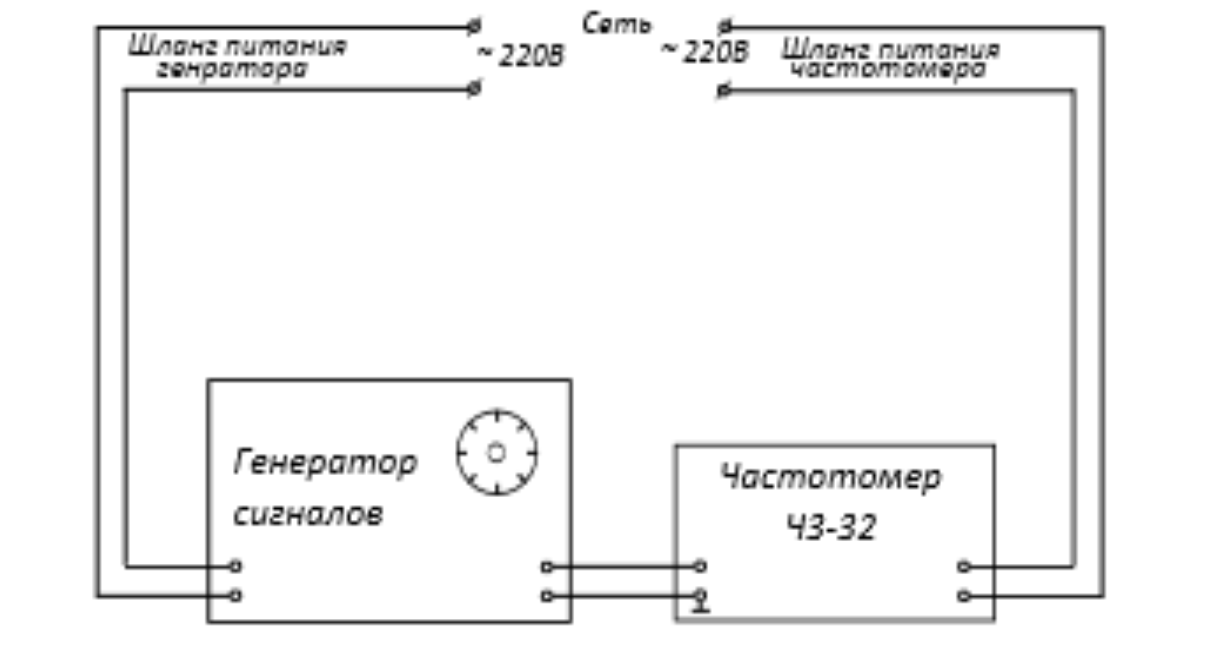
\includegraphics[width=0.8\textwidth]{scheme.png}
\caption{Блок-схема экспериментальной установки}
\end{figure}

\textbf{Эксперимент проводился в следующей последовательности:}

\begin{enumerate}
\item Ознакомление с работой частотомера и выбор шкалы для измерения периода.
\item Измерение периода следования импульсов на грубой шкале прибора (диапазон $10^{-6}$).
\item Переключение шкалы частотометра с грубой на точную.
\item Проведение серии измерений по точной шкале прибора (диапазон $10^{-4}$).
\item Запись результатов измерений в таблицы для последующей обработки.
\end{enumerate}

\subsection{Обработка результатов измерений}

По результатам серии измерений определялось среднее значение периода следования импульсов.

Среднее значение периода вычислялось по формуле:

\begin{equation}
\overline{T} = \frac{1}{n}\sum_{i=1}^{n} T_i,
\end{equation}

где \(T_i\) — результаты отдельных измерений, \(n\) — число измерений.

\begin{equation}
\overline{T} = 273,389 \; \text{мс},
\end{equation}
среднее значение периода, полученное на основе обработки резултатов полученных с точной шкалы.

Далее все графики и таблицы строятся на основе результатов, полученных с точной шкалы.

Проверялось не изменяется ли измеряемая величина регулярным образом с течением времени. Для этого строился график зависимости результатов наблюдений от времени.

\begin{figure}[H]
\centering
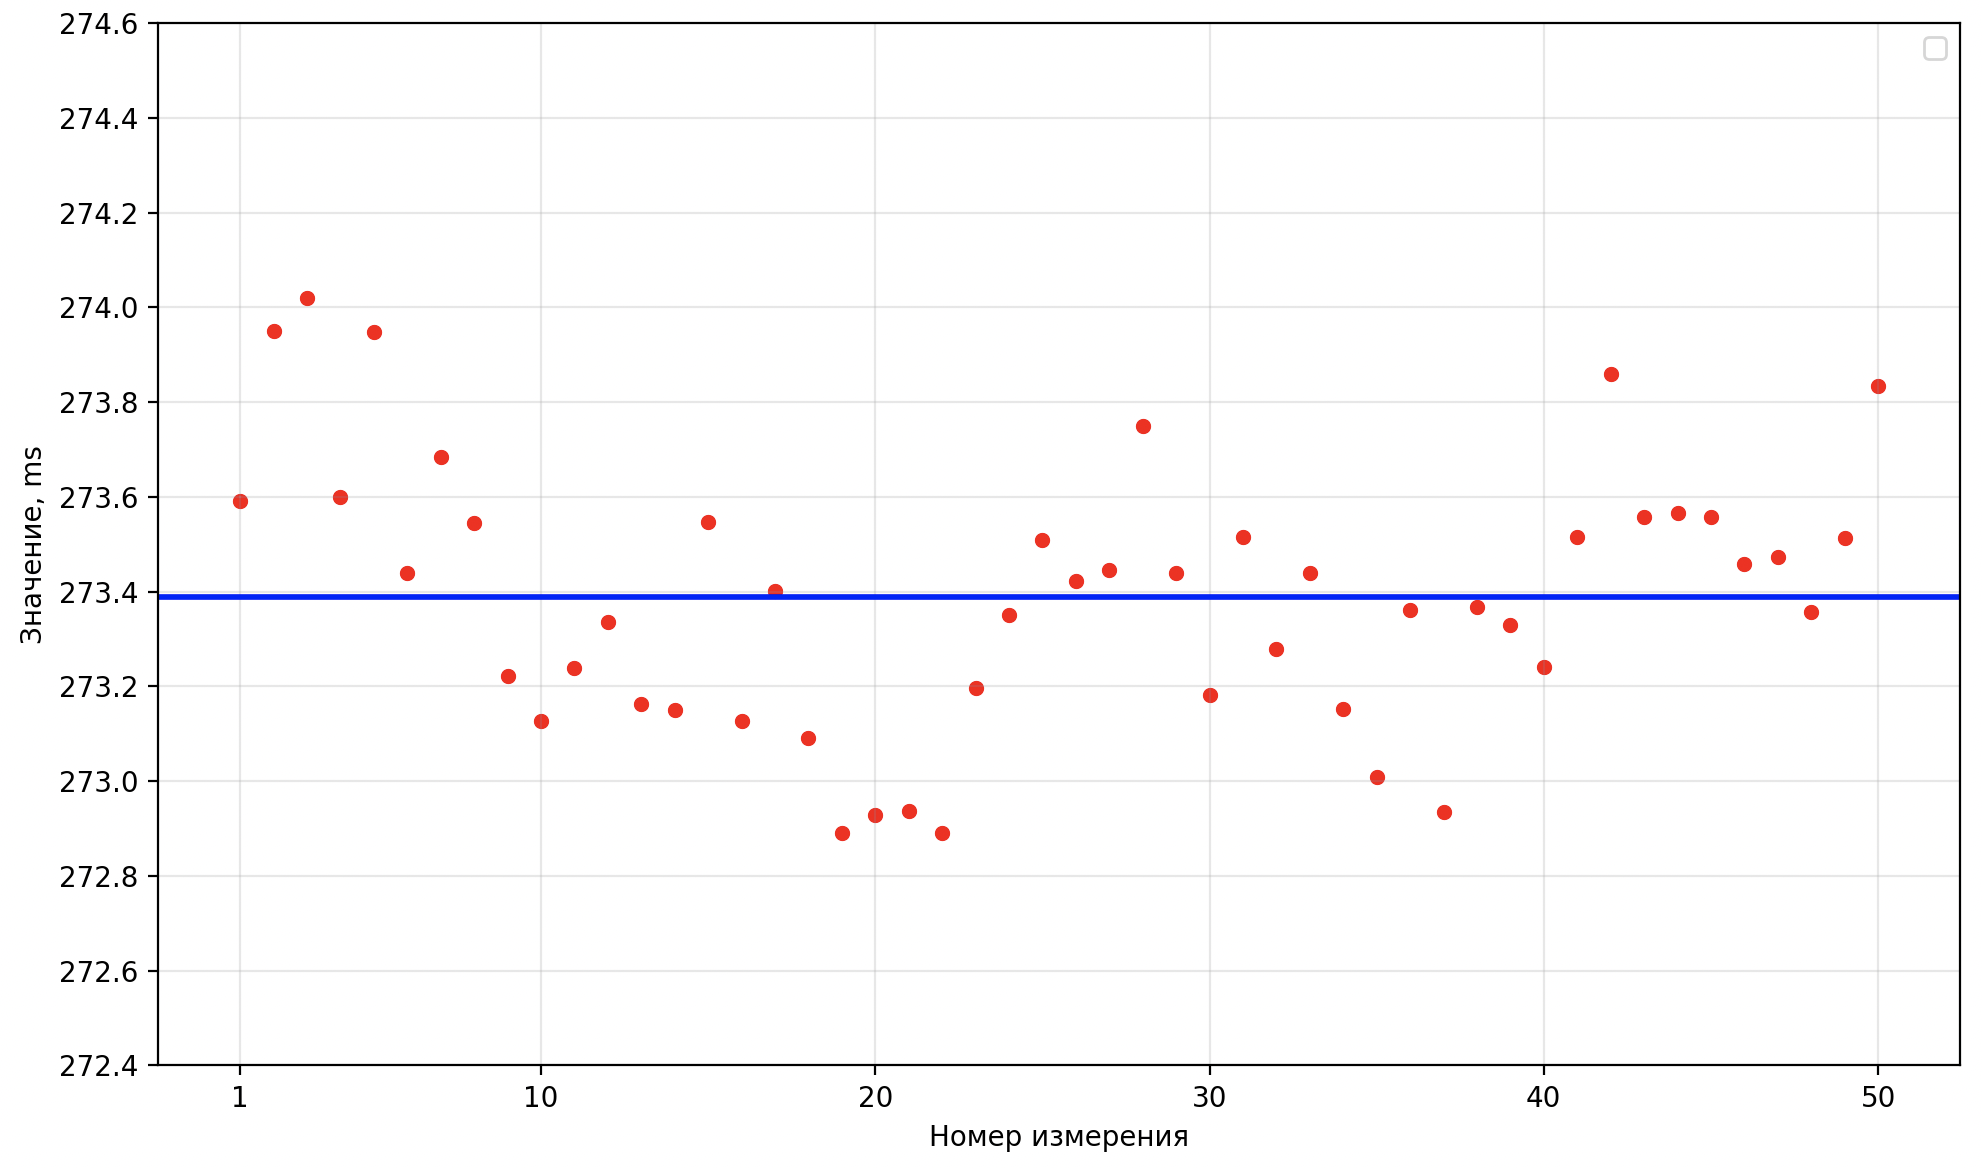
\includegraphics[width=0.8\textwidth]{g1.png}
\caption{Зависимость результатов наблюдений от времени}
\end{figure}

На основании построенного графика было установлено, что дрейф отсутствует, следовательно можно переходить к построению гистограммы.

Для начала на числовую ось наносились все результаты отдельных
наблюдений и установливался диапазон, в котором находились все полученные результаты наблюдений.
\begin{figure}[H]
\centering
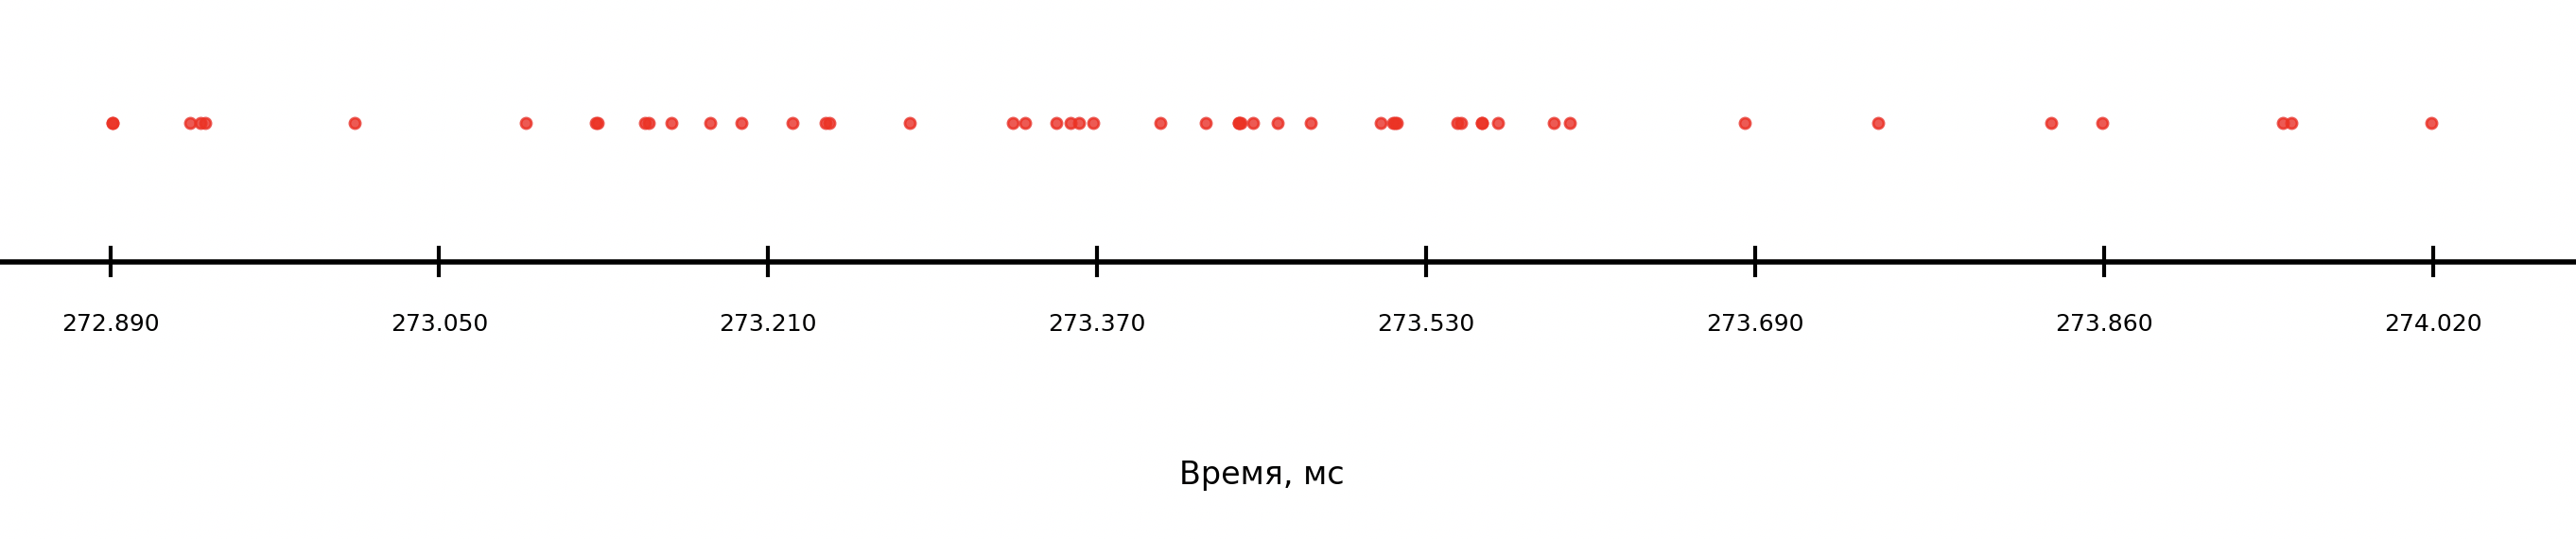
\includegraphics[width=\textwidth, height=4cm]{dot.png}
\caption{Результаты наблюдений на числовой оси}
\end{figure}

Далее были определены Tmin = 272,891 мс и Tmax = 274,019 мс. Диапозон был разбит на 7 интервалов с шагом 0,160 мс.

\begin{table}[H]
\centering
\caption{Результаты группировки измерений времени}
\begin{tabular}{|c|c|c|c|}
\hline
\begin{tabular}{c} Номер \\ интервала \end{tabular} & \begin{tabular}{c} Границы интервалов \\ ($\Delta t = 0,161$ мс) \end{tabular} & \begin{tabular}{c} Число случаев \\ ($\Delta n$) \end{tabular} & \begin{tabular}{c} Доля \\ ($\delta = \Delta n / n$) \end{tabular} \\
\hline
1 & 272,890 - 273,051 & 7 & 0,140 \\
\hline
2 & 273,051 - 273,212 & 7 & 0,140 \\
\hline
3 & 273,212 - 273,373 & 10 & 0,200 \\
\hline
4 & 273,373 - 273,534 & 11 & 0,220 \\
\hline
5 & 273,534 - 273,695 & 8 & 0,160 \\
\hline
6 & 273,695 - 273,856 & 3 & 0,060 \\
\hline
7 & 273,856 - 274,017 & 3 & 0,060 \\
\hline
\multicolumn{3}{|r|}{Всего:} & \multicolumn{1}{c|}{1,000} \\
\hline
\end{tabular}
\end{table}
На основании таблицы строилась гистограмма
\begin{figure}[H]
\centering
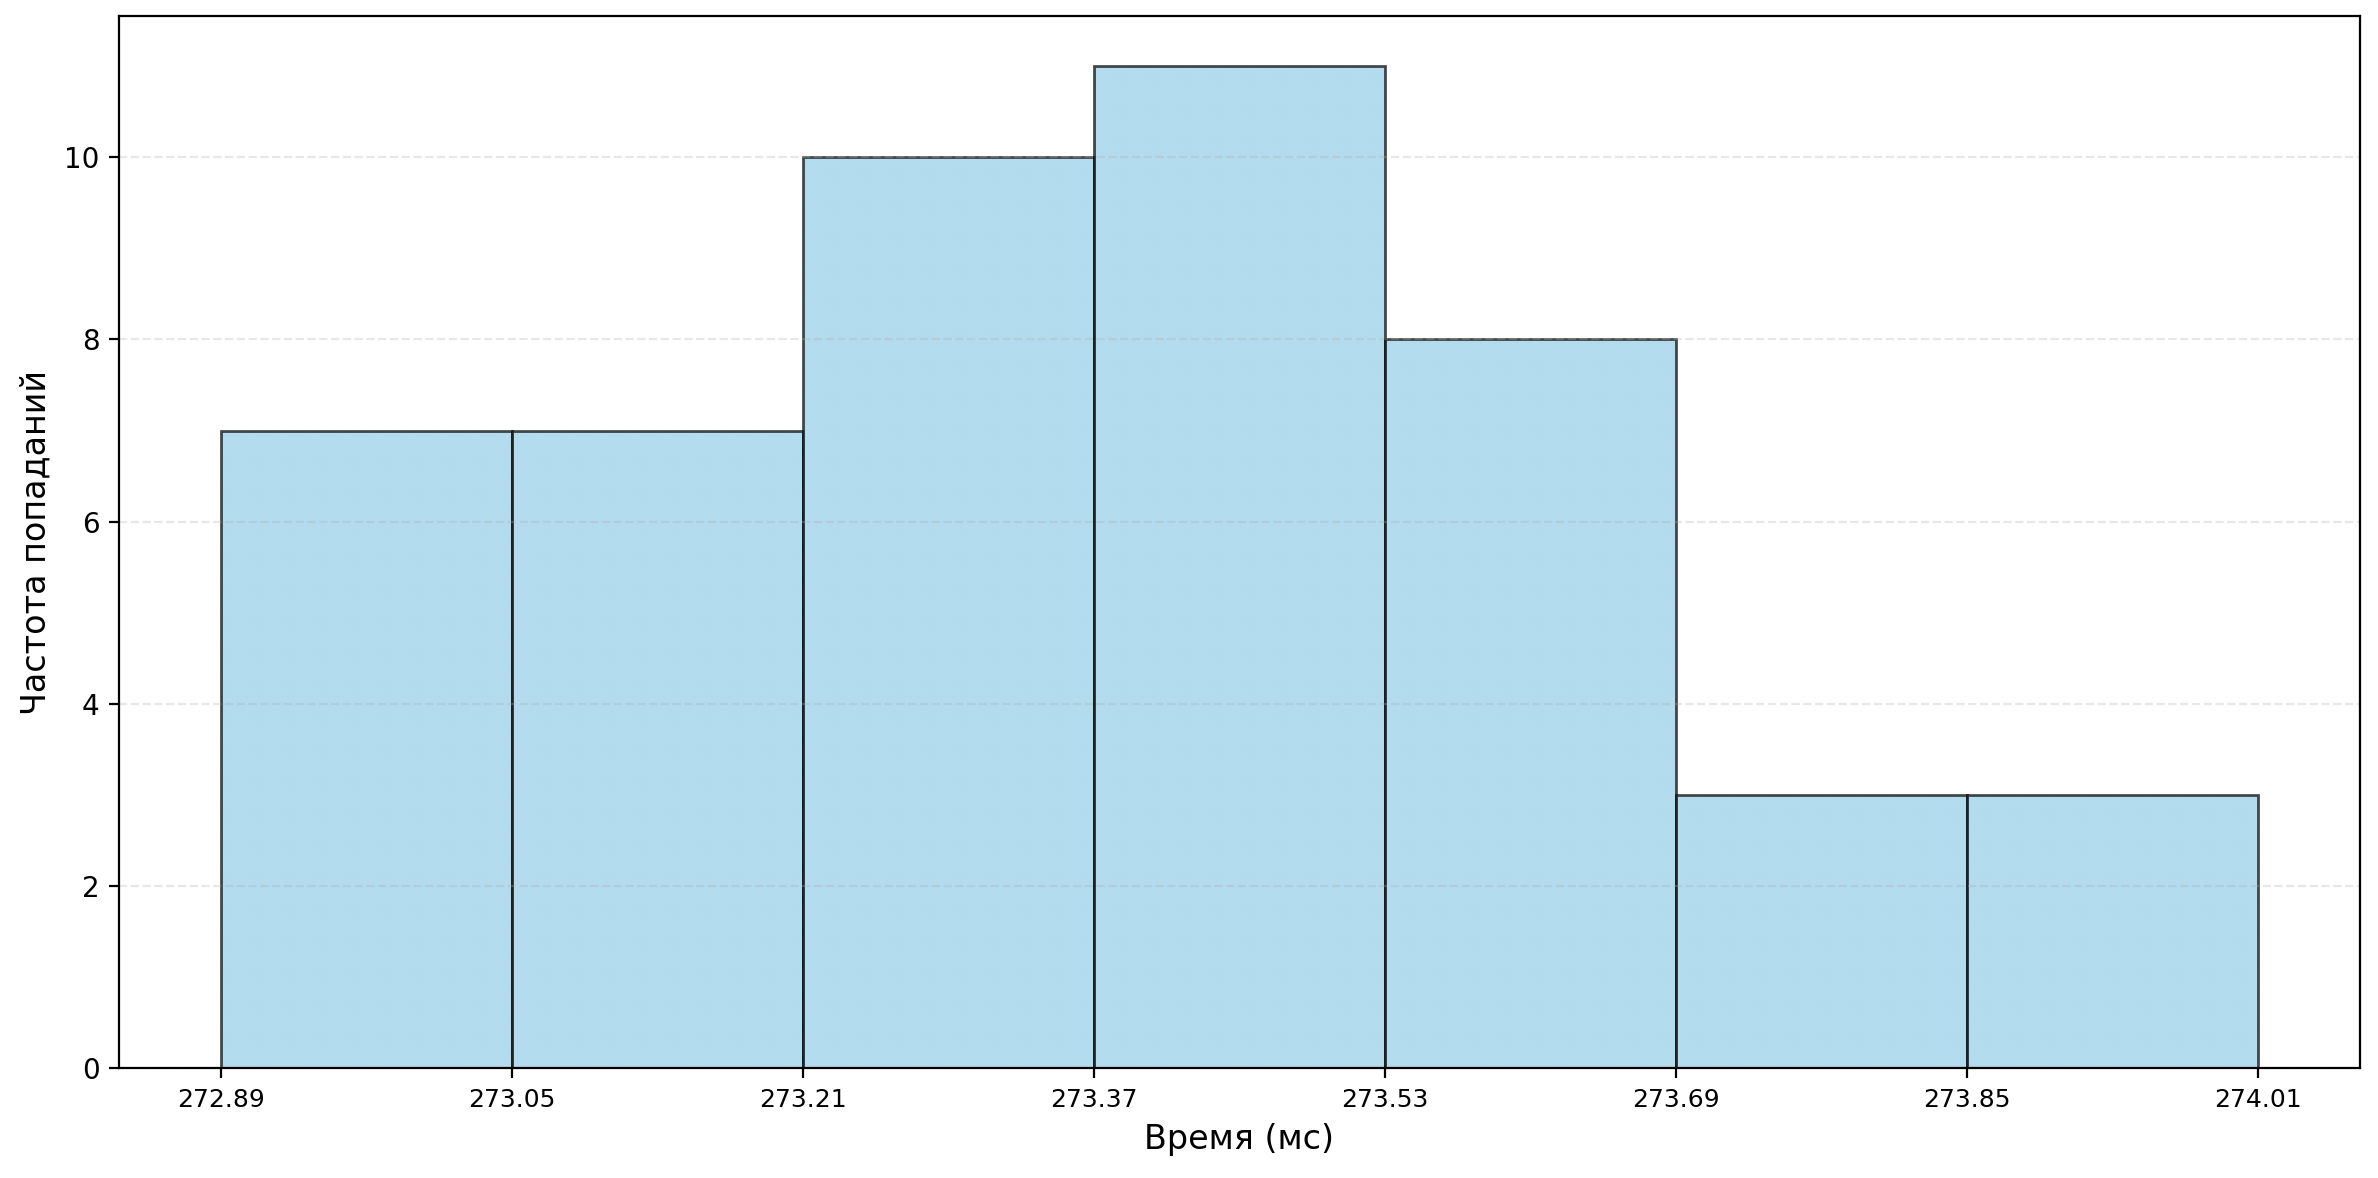
\includegraphics[width=0.8\textwidth]{histogram.png}
\caption{Гистограмма}
\end{figure}
И график плотности распределения
\begin{figure}[H]
\centering
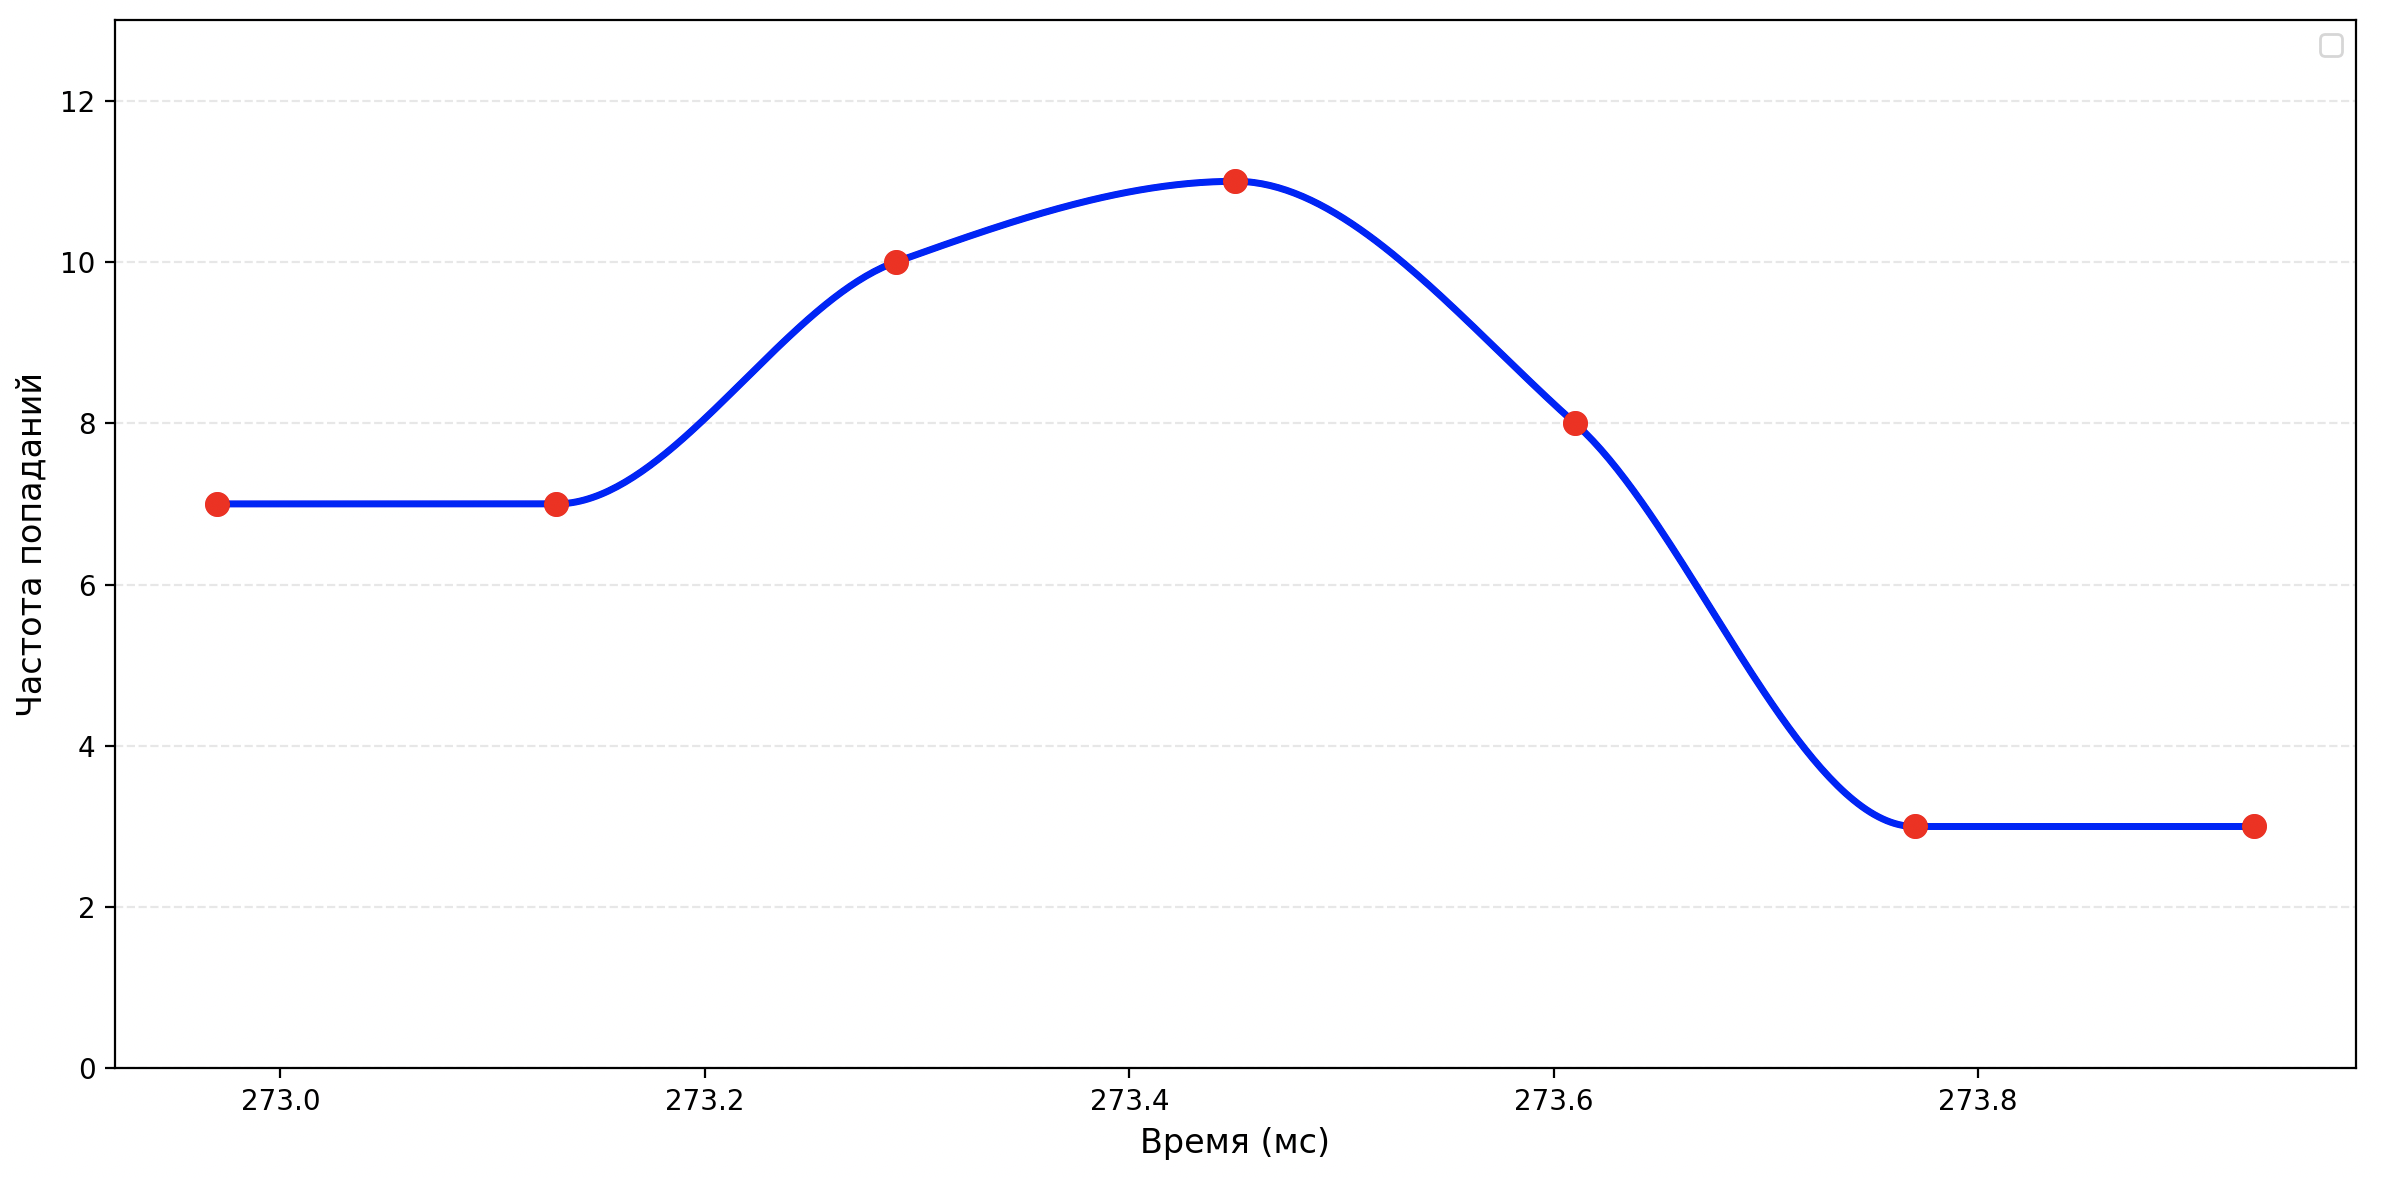
\includegraphics[width=0.8\textwidth]{curve.png}
\caption{График зависимости}
\end{figure}
Для оценки разброса результатов рассчитывалось среднеквадратичное отклонение:

\begin{equation}
\sigma = \sqrt{\frac{1}{n-1}\sum_{i=1}^{n}(T_i - \overline{T})^2}.
\end{equation}

\begin{equation}
\sigma = 0,278
\end{equation}

На основании полученных данных вычислялась оценка средней квадратичной погрешности измерения

\begin{equation}
\sigma_{x} = \sigma/\sqrt{n}
\end{equation}

\begin{equation}
\sigma_{x} = 0,039
\end{equation}
и результат записывался в виде:

\[
T = \overline{T} \pm \Delta T.
\]
\begin{equation}
T = 273,389 \pm 0,039 \; \text{мс}
\end{equation} \text{мс}

Для того чтобы оценить точность результатов, было проведено сравнение погрешности прибора $\Delta T = 0,0011$ мс со случайной погрешностью $\sigma_{x} = 0,039$. Поскольку случайная погрешность превышает приборную в 35 раз, сделан вывод о том что основной вклад вносит случайная погрешность.

\section{Выводы}

В ходе работы были проведены измерения электромеханических характеристик. В ходе эксперимента установлено, что случайная погрешность измерений ($\sigma_{x} = 0,039$) превышает приборную погрешность частотомера ($\Delta T = 0,0011$ мс). 
Это говорит о том, что основной вклад в общую погрешность вносят случайные факторы. 

Приборная погрешность оказывается пренебрежимо малой по сравнению с разбросом результатов, что подтверждается формой гистограммы — она близка к нормальному распределению, характерному для случайных процессов. Уменьшить погрешность можно только увеличением числа наблюдений, но не заменой прибора.
\clearpage
\appendix
\end{document}


